
\subsubsection{投影与相机模型}

\begin{figure}[H]
    \centering
    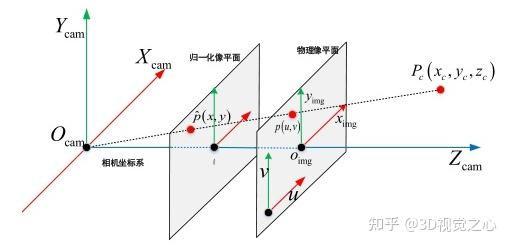
\includegraphics[width=0.8\linewidth]{相机模型.jpg}
    \caption{相机成像过程：CMOS应该位于透镜后，图中作了修改以便于理解}
    \label{fig:camera}
\end{figure}

相机成像的过程可以简单的看做是一个投影的过程，如图\ref{fig:camera}所示。
相机成像的核心是一个CMOS传感器，其上分布有许多区域，对应着图像中的一个像素点。
当光线通过相机镜头时，会在CMOS传感器上形成一个像素点的亮斑，这个亮斑的中心位置就是图像中的一个像素点。

CMOS传感器是一个平面，被称为\textbf{成像平面}，距离镜头光心的距离被称为\textbf{焦距}。
应用相似三角形的原理，可以进行投影变换。

\begin{equation}
    \begin{aligned}
        \frac{X}{Z} &= \frac{U}{f_x} \\
        \frac{Y}{Z} &= \frac{V}{f_y}
    \end{aligned}
\end{equation}

我们一般将图像坐标系的原点设置在图像的角，需要给方程添加一个偏移量，写成矩阵形式就是：

\begin{equation}
    \begin{bmatrix}
        U \\
        V
    \end{bmatrix} =
    \begin{bmatrix}
        f_x & 0 \\
        0 & f_y
    \end{bmatrix}
    \begin{bmatrix}
        X/Z \\
        Y/Z
    \end{bmatrix} +
    \begin{bmatrix}
        c_x \\
        c_y
    \end{bmatrix}
\end{equation}

做一下维数统一，引入\textbf{齐次坐标}：

\begin{equation}
    \begin{bmatrix}
        U \\
        V \\
        1
    \end{bmatrix} = \frac{1}{Z}
    \begin{bmatrix}
        f_x & 0 & c_x \\
        0 & f_y & c_y \\
        0 & 0 & 1
    \end{bmatrix}
    \begin{bmatrix}
        X \\
        Y \\
        Z
    \end{bmatrix}
\end{equation}

这就是最基本的相机模型。

\begin{example}
无畸变针孔模型中，fx=fy=800、cx=320、cy=240，相机坐标 (0.2,0.1,2) m 投影为 (400,280) pixel。
\begin{tpython}
fx,fy,cx,cy=800,800,320,240
X,Y,Z=0.2,0.1,2.0
u,v=fx*X/Z+cx,fy*Y/Z+cy
assert (u,v)==(400,280)
print(u,v)
\end{tpython}
\end{example}

\begin{exercise}
把距离 Z 加倍，计算新的像素坐标。说明像素坐标为何不是简单除以 2。
\end{exercise}

\subsubsection{相机内参与标定}

实际中镜头并不是理想的，会产生畸变，所以仅直到焦距这些数据并不足以完整地描述相机成像过程中的坐标变换关系。
引入畸变矩阵$\mathbf{D}$，使其与原来的投影矩阵$\mathbf{C}$相乘，得到内参矩阵$\mathbf{K}$：

\begin{equation}
    \begin{bmatrix}
        U \\
        V \\
        1
    \end{bmatrix} = \frac{1}{Z} \mathbf{K}
    \begin{bmatrix}
        X \\
        Y \\
        Z
    \end{bmatrix}
\end{equation}

我们不对畸变矩阵进行过多的讨论，对于畸变的产生和消除也不做过多的探讨，因为其与当前主题无关，
主要关注于内参矩阵$\mathbf{K}$的标定。

\begin{figure}[H]
    \centering
    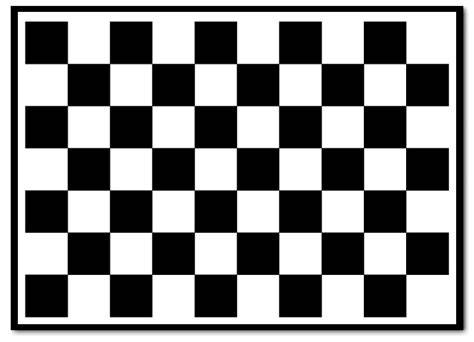
\includegraphics[width=0.8\linewidth]{标定板.jpeg}
    \caption{相机标定：\textbf{一般采用张正友标定法}}
    \label{fig:calibration}
\end{figure}

使用ROS的calibration包可以很方便地进行相机标定，标定的过程主要是通过拍摄一系列不同位置和姿态的标定板（如图\ref{fig:calibration}所示），来计算出相机的内参矩阵$\mathbf{K}$。
标定的结果包括焦距、主点位置和畸变参数等，这些参数对于后续的图像处理和空间位置解算非常重要。

\begin{example}
原图 640×480，fx=800、cx=320。仅进行各方向等比例 0.5 缩放且不裁剪时，fx 变为 400、cx 变为 160；标准归一化畸变系数保持不变。若裁剪左侧 20 pixel，主点还要相应平移。
\end{example}

\begin{exercise}
原图 fy=820、cy=240，缩小到一半后再从顶部裁去 10 pixel，求新的 fy 与 cy。
\end{exercise}

\subsubsection{坐标系变换与相机外参}
除了相机成像的过程，要想实现自瞄系统，就需要对目标进行空间位置解算，这就需要引入坐标系变换的概念。

\paragraph*{三维空间刚体运动}
三维空间中，通过设置一组基向量$[\mathbf{e_1},\mathbf{e_2},\mathbf{e_3}]$，就可以通过线性变换表示这个空间中任意一个点的位置。
\begin{equation}
    \mathbf{a} = [\mathbf{e_1},\mathbf{e_2},\mathbf{e_3}] [a_1, a_2, a_3]^T
\end{equation}

$[a_1, a_2, a_3]^T$是点$\mathbf{a}$在此基下的坐标。

现在来分析坐标系之间的关系，$\mathbf{P}$分解在两个坐标系下。

\begin{equation}
    \mathbf{P} = [\mathbf{e_1},\mathbf{e_2},\mathbf{e_3}] 
    \begin{bmatrix}
        a_1 \\
        a_2 \\
        a_3
    \end{bmatrix}
    = [\mathbf{e_1'},\mathbf{e_2'},\mathbf{e_3'}] 
    \begin{bmatrix}
        a_1' \\
        a_2' \\
        a_3'
    \end{bmatrix}
\end{equation}

在两边乘上$[\mathbf{e_1},\mathbf{e_2},\mathbf{e_3}]^{-1}$，
也就是 $[\mathbf{e_1},\mathbf{e_2},\mathbf{e_3}]^T$
得到：

\begin{equation}
    \begin{bmatrix}
        a_1 \\
        a_2 \\
        a_3
    \end{bmatrix}
    =
    \begin{bmatrix}
        \mathbf{e_1}^T \mathbf{e_1'} & \mathbf{e_1}^T \mathbf{e_2'} & \mathbf{e_1}^T \mathbf{e_3'} \\
        \mathbf{e_2}^T \mathbf{e_1'} & \mathbf{e_2}^T \mathbf{e_2'} & \mathbf{e_2}^T \mathbf{e_3'} \\
        \mathbf{e_3}^T \mathbf{e_1'} & \mathbf{e_3}^T \mathbf{e_2'} & \mathbf{e_3}^T \mathbf{e_3'}
    \end{bmatrix}
    \begin{bmatrix}
        a_1' \\
        a_2' \\
        a_3'
    \end{bmatrix}
    \overset{\text{def}}{=}
    \mathbf{R}\mathbf{a'}
\end{equation}

这里的$\mathbf{R}$就是坐标系之间的\textbf{旋转矩阵}，描述了两个坐标系之间的旋转关系。
旋转矩阵还有一些特别的性质，他是一个行列式为1的正交矩阵，可以对n维旋转矩阵进行下面的定义：
\begin{equation}
    SO(n) = \{\mathbf{R} \in \mathbb{R}^{n \times n} | \mathbf{R}^T\mathbf{R} = \mathbf{I}, \det(\mathbf{R}) = 1\}
\end{equation}
$SO(n)$是\textbf{特殊正交群}，描述了n维空间中的旋转变换。$SO(3)$表示三维空间中的旋转变换。
$R^T$ 刻画了一个相反的旋转关系，因为$R^{-1} = R^T$。

欧式变换中，除了旋转之外还有平移。$a$经过一次旋转$R$和平移$t$之后得到$a'$，可以表示为：
\begin{equation}
    \mathbf{a'} = \mathbf{R}\mathbf{a} + \mathbf{t}
\end{equation}

这里还有一个问题，这个变换不是线性的，我们可以通过引入\textbf{齐次坐标}来将其转化为线性变换。
\begin{equation}
    \begin{bmatrix}
        a' \\
        1
    \end{bmatrix} =
    \begin{bmatrix}
        \mathbf{R} & \mathbf{t} \\
        \mathbf{0}^T & 1
    \end{bmatrix}
    \begin{bmatrix}
        a \\
        1
    \end{bmatrix}
    \overset{\text{def}}{=}
    \mathbf{T}[\mathbf{a},1]^T
\end{equation}

$\mathbf{T}$被称为\textbf{变换矩阵}，描述了两个坐标系之间的旋转和平移关系。

\begin{equation}
    SE(n) = \{\mathbf{T}|\mathbf{T} = 
    \begin{bmatrix}
        \mathbf{R} & \mathbf{t} \\
        \mathbf{0}^T & 1
    \end{bmatrix}, \mathbf{R} \in SO(n), \mathbf{t} \in \mathbb{R}^n\}
\end{equation}

$SE(n)$被称为\textbf{特殊欧式群}，描述了n维空间中的旋转和平移变换。$SE(3)$表示三维空间中的旋转和平移变换。
与$SO(3)$类似，$SE(3)$也有一个相反的变换关系，可以通过求逆来得到：
\begin{equation}
    \mathbf{T}^{-1} =
    \begin{bmatrix}
        \mathbf{R}^T & -\mathbf{R}^T\mathbf{t} \\
        \mathbf{0}^T & 1
    \end{bmatrix}
\end{equation}

也可以简写成 $\mathbf{a}' = \mathbf{Ta}$ ，这里隐含一个齐次坐标与非齐次坐标的转换，并不是简单的矩阵乘法，否则是不成立的。
这种表述后文也会出现，不再赘述。

SO(n)和SE(n)是李群，具有连续性和平滑性，可以通过指数映射和对数映射在李代数和李群之间进行转换。
这些性质在~\ref{sec:李代数}中会有简要的介绍。

\paragraph*{自瞄系统的常见坐标系}
在自瞄系统中，常见的坐标系主要有以下几种：

\textbf{图像坐标系：} 图像坐标系是以图像中心为原点，x轴和y轴分别指向图像的右侧和下方的坐标系，z轴指向图像平面的法线方向.

\textbf{相机坐标系：} 相机坐标系是以相机光心为原点，z轴指向相机前方，x轴和y轴分别指向相机的右侧和下方的坐标系，原点在相机成像平面中心.

\textbf{云台系：} 云台系是以云台旋转中心为原点，x轴指向云台前方，y轴和z轴分别指向云台的右侧和上方的坐标系，圆点在云台旋转中心.

\textbf{世界坐标系：} 自瞄系统的世界系指的是，上电初始位置的云台坐标系，但是不与云台绑定，始终保持不变.

\paragraph*{相机外参}

指的是描述相机坐标系与世界坐标系之间关系的变换矩阵$\mathbf{T}$，它包含了旋转和平移两个部分。
一般来说，相机的位态都可以称为相机外参，一般是相对于世界系的，但是在不同的应用场景和需求下，也不绝对。

\begin{example}
列向量约定下，R 为单位阵，t=(1,0,0)。物体点 (0,2,3) 变到相机系为 (1,2,3)；逆变换应恢复原点坐标。需要 NumPy。
\begin{tpython}
import numpy as np
R=np.eye(3); t=np.array([1.,0.,0.])
p=np.array([0.,2.,3.])
q=R@p+t
recovered=R.T@(q-t)
assert np.allclose(q,[1,2,3]) and np.allclose(recovered,p)
print(q,recovered)
\end{tpython}
\end{example}

\begin{exercise}
绕 z 轴旋转 90°，平移不变，手算并修改 R 验证结果。
\end{exercise}

\subsubsection{PnP问题与求解}

PnP问题是指在已知空间中n个点的坐标以及它们在图像中的投影位置的情况下，求解相机的位姿（位置和姿态）的问题。

\paragraph*{直接线性变换DLT}

直接考虑这样一个问题：已知一组3D点的位置，以及他们在某个相机中的投影位置，求解该相机的位姿。

考虑某个空间点$\mathbf{P}=(X, Y, Z)^T$，在图像中特征点$\mathbf{p}=(u_1, v_1,1)^T$。
我们定义一个增广矩阵$[\mathbf{R} | \mathbf{t}]$，有$\mathbf{p} = [\mathbf{R} | \mathbf{t}] \mathbf{P}$，
展开来写就是：

\begin{equation}
    d\begin{bmatrix}
        u_1 \\
        v_1 \\
        1
    \end{bmatrix}
    =
    \begin{bmatrix}
        t_{1} & t_{2} & t_{3} & t_4 \\
        t_{5} & t_{6} & t_{7} & t_8 \\
        t_{9} & t_{10} & t_{11} & t_12
    \end{bmatrix}
    \begin{bmatrix}
        X \\
        Y \\
        Z \\
        1
    \end{bmatrix}
\end{equation}

使用最后一行把$d$消掉，得到两个约束：

\begin{equation}
    \begin{aligned}
        u_1 = \frac{t_1X+t_2Y+t_3Z+t_4}{t_9X+t_{10}Y+t_{11}Z+t_{12}} \\
        v_1 = \frac{t_5X+t_6Y+t_7Z+t_8}{t_9X+t_{10}Y+t_{11}Z+t_{12}} 
    \end{aligned}
\end{equation}

做一些简化表示：

\begin{equation}
    \begin{aligned}
        \mathbf{t_1} = (t_1,t_2,t_3,t_4)^T \\
        \mathbf{t_2} = (t_5,t_6,t_7,t_8)^T \\
        \mathbf{t_3} = (t_9,t_{10},t_{11},t_{12})^T
    \end{aligned}
\end{equation}

于是有：

\begin{equation}
    \begin{aligned}
        \mathbf{t_1}^T\mathbf{P} - \mathbf{t_3}^T\mathbf{P}u_1 = 0 \\
        \mathbf{t_2}^T\mathbf{P} - \mathbf{t_3}^T\mathbf{P}v_1 = 0  
    \end{aligned}
\end{equation}

$\mathbf{t}$是待求的变量，可以看到，每个特征点可以提供两个方程，至少需要6个特征点就可以求解出$\mathbf{t}$。

\begin{equation}
    \begin{bmatrix}
        \mathbf{P_1}^T & \mathbf{0}^T & -u_1\mathbf{P_1}^T \\
        \mathbf{0}^T & \mathbf{P_1}^T & -v_1\mathbf{P_1}^T \\
        \vdots & \vdots & \vdots \\
        \mathbf{P_n}^T & \mathbf{0}^T & -u_n\mathbf{P_n}^T \\
        \mathbf{0}^T & \mathbf{P_n}^T & -v_n\mathbf{P_n}^T
    \end{bmatrix}
    \begin{bmatrix}
        \mathbf{t_1} \\
        \mathbf{t_2} \\
        \mathbf{t_3}
    \end{bmatrix} = \mathbf{0}
\end{equation}

这种方法被称为\textbf{直接线性变换DLT}。当匹配点的数量大于6时，可以通过$SVD$等方法对超定方程求最小二乘解。

在DLT求解中，我们忽略了$\mathbf{T}$的各元素关系。旋转矩阵$R \in SO(3)$，DLT求解得到的$\mathbf{T}$不一定满足这个约束，所以需要对求解结果进行后续处理，来满足旋转矩阵的约束。
若内参已知，先恢复旋转部分并消除尺度，再做旋转投影。满秩时可用极分解，例如：

\begin{equation}
    \mathbf{R} \gets (\mathbf{R}\mathbf{R}^T)^{-\frac{1}{2}}\mathbf{R}
\end{equation}

内外参分离与旋转投影的区别见后文(参考~\ref{sec:DLT的QR求解} 和~\ref{sec:DLT的极分解求解})。

\paragraph*{P3P}

P3P是另一种求解PnP问题的方法，它仅使用三对匹配点，对数据要求较少。

\begin{figure}[H]
    \centering
    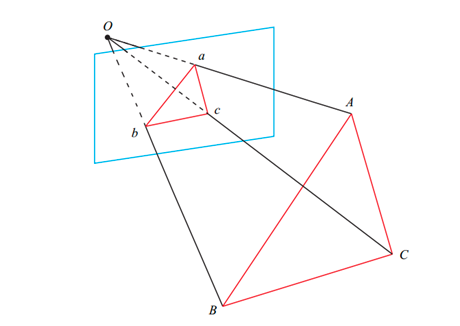
\includegraphics[width=0.99\linewidth]{p3p.png}
    \caption{P3P求解示意图}
    \label{fig:P3P}
\end{figure}

以图~\ref{fig:P3P}为例，已知空间中三个点$A, B, C$的位置，以及它们在图像中的投影位置$a, b, c$，求解相机的位姿。

显然存在一些几何上的相似关系：
\begin{equation}
    \begin{aligned}
        \bigtriangleup Oab \sim \bigtriangleup OAB \\
        \bigtriangleup Obc \sim \bigtriangleup OBC \\
        \bigtriangleup Oca \sim \bigtriangleup OCA
    \end{aligned}
\end{equation}

列写余弦定理的方程：
\begin{equation}
    \begin{aligned}
        OA^2 +OB^2 -2OA\cdot OB \cdot \cos<a,b> = AB^2 \\
        OB^2 +OC^2 -2OB\cdot OC \cdot \cos<b,c> = BC^2 \\
        OC^2 +OA^2 -2OC\cdot OA \cdot \cos<c,a> = CA^2
    \end{aligned}
\end{equation}

令$x = \frac{OA}{OC}, y = \frac{OB}{OC}$，全体除以$OC^2$，得到：
\begin{equation}
    \begin{aligned}
        x^2 + y^2 - 2xy\cos<a,b> = \frac{AB^2}{OC^2} \\
        y^2 + 1 - 2y\cos<b,c> = \frac{BC^2}{OC^2} \\
        1 + x^2 - 2x\cos<c,a> = \frac{CA^2}{OC^2}
    \end{aligned}
\end{equation}

记$v=\frac{AB^2}{OC^2}$，$uv=\frac{BC^2}{OC^2}$，$wv=\frac{AC^2}{OC^2}$，得到：
\begin{equation}
    \begin{aligned}
        x^2 + y^2 - 2xy\cos<a,b> - v = 0 \\
        y^2 + 1 - 2y\cos<b,c> - uv = 0 \\
        x^2 + 1 - 2x\cos<c,a> - wv = 0
    \end{aligned}
\end{equation}

将第一个式子的$v$带入第二、三个式子，得到：
\begin{equation}
    \begin{aligned}
        (1-u)y^2 - ux^2 - y\cos<b,c> + 2uxy\cos<a,b> + 1 = 0 \\
        (1-w)x^2 - wy^2 - x\cos<a,c> + 2wxy\cos<a,b> + 1 = 0
    \end{aligned}
\end{equation}

重新审视这个方程组，由于我们知道2D点的图像位置，所以可以计算出<a,b>、<b,c>、<c,a>的值，
空间点的位置也已知，所以可以计算出$u$和$w$的值。
所以事实上是一个关于$x,y$的二元二次方程。

这个方程的解析解求解过程非常复杂，需要用到吴消元法，在此不再讨论。
计算得到$x,y,v$的值就可以推算出$OA,OB,OC$的值，也就是计算出了相机系下的点坐标，我们称之为3D-3D点对，转换为了ICP问题，
从而可以求解出相机的位姿。ICP求解相较于PnP是比较简单的，具体方法可以参考~\ref{sec:ICP求解}。

P3P也存在一些问题：
\begin{itemize}
    \item P3P只利用3个点的信息。当给定的配对点多余3组时，难以利用多余的信息
    \item 如果3D点或2D点存在噪声，或存在误匹配，则算法失效
\end{itemize}

\begin{example}
用已知位姿合成八个非共面的点，再调用 solvePnP 恢复。Python 环境需 numpy 与 opencv-python。无噪声时重投影均方根误差应小于 0.001 pixel。
\begin{tpython}
import cv2
import numpy as np
obj=np.array([[x,y,z] for x in [-.1,.1] for y in [-.1,.1]
              for z in [0.,.2]],dtype=np.float64)
K=np.array([[800.,0,320],[0,800,240],[0,0,1]])
dist=np.zeros(5)
r=np.array([.1,.2,0.]); t=np.array([0.,0.,2.])
image,_=cv2.projectPoints(obj,r,t,K,dist)
ok,r_hat,t_hat=cv2.solvePnP(obj,image,K,dist,flags=cv2.SOLVEPNP_ITERATIVE)
if not ok: raise RuntimeError("PnP 求解失败")
reprojected,_=cv2.projectPoints(obj,r_hat,t_hat,K,dist)
rms=np.sqrt(np.mean(np.sum((reprojected-image)**2,axis=2)))
assert rms < 1e-3
print(t_hat.ravel(),rms)
\end{tpython}
\end{example}

\begin{exercise}
打乱两个二维点的对应顺序，比较误差。说明只看求解函数返回成功为何不够。
\end{exercise}

\begin{note}
solvePnP 输出把物体系点变到相机系的旋转和平移。点数要求取决于解法；共面、共线与错误对应都可能造成歧义或退化。
\end{note}

\subsubsection{最小化重投影误差BA}

除了使用线性方法，还可以把PnP问题构建成一个关于重投影误差的非线性最小二乘问题。
可以用它对PnP或ICP的结果进行优化，得到更准确的位姿估计。
这一类把相机和三维点放在一起优化的问题，统称为\textbf{Bundle Adjustment}，简称BA。

\paragraph*{问题引入}

考虑\(n\)个三维空间点\(P\)和它们的投影\(p\)，我们希望基于此计算相机位姿。假设某点\(\mathbf{P}\_i=[X\_i,Y\_i,Z\_i]^T\)，其投影\(\mathbf{p}\_i=[u\_i,v\_i]^T\)，相机位姿的李群表示为\(\mathbf{T}\)。它们的空间位置关系可以表示为：
\begin{equation}
    s_i\begin{bmatrix}
        u_i \\
        v_i \\
        1
    \end{bmatrix}
    =
    \mathbf{K}\mathbf{T}
    \begin{bmatrix}
        X_i \\
        Y_i \\
        Z_i \\
        1
    \end{bmatrix}
\end{equation}

也就是：
\begin{equation}
    s_i\mathbf{p}_i = \mathbf{K}\mathbf{T}\mathbf{P}_i
\end{equation}

由于噪声存在，上面的这个等式不再成立，可以让它的两边的差距最小化，得到一个非线性最小二乘问题，求解最优的\(\mathbf{T}\)：
\begin{equation}
    \mathbf{T}^* = \arg\min_{\mathbf{T}} \frac{1}{2}\sum_{i=1}^n \|s_i\mathbf{p}_i - \mathbf{K}\mathbf{T}\mathbf{P}_i\|^2_2
\end{equation}

更一般地，设\(z\_{ij}\)为在位姿\(\boldsymbol{\xi}\_i\)处观察路标\(\mathbf{p}\_j\)产生的像素坐标，观测方程抽象为：
\begin{equation}
    z_{ij} = h(\boldsymbol{\xi}_i, \mathbf{p}_j)
\end{equation}
其中\(\boldsymbol{\xi}\_i\)为相机位姿\(\mathbf{T}\_i\)对应的李代数。观测误差定义为：
\begin{equation}
    \mathbf{e}_{ij} = z_{ij} - h(\boldsymbol{\xi}_i, \mathbf{p}_j)
\end{equation}

将相邻时刻的观测全部考虑进来，整体的BA代价函数为：
\begin{equation}\label{eq:ba_cost}
    F(\mathbf{x}) = \frac{1}{2}\sum_{i=1}^m\sum_{j=1}^n \|\mathbf{e}_{ij}\|^2
    = \frac{1}{2}\sum_{i=1}^m\sum_{j=1}^n \|z_{ij} - h(\boldsymbol{\xi}_i, \mathbf{p}_j)\|^2
\end{equation}
其中\(\mathbf{x} = [\boldsymbol{\xi}\_1, \dots, \boldsymbol{\xi}\_m, \mathbf{p}\_1, \dots, \mathbf{p}\_n]^T\)为所有待优化的变量，包括所有相机位姿和三维路标点。对这个最小二乘进行求解，相当于对位姿和路标同时进行调整，这就是BA。

\paragraph*{求解方法}

观测模型\(h(\boldsymbol{\xi}, \mathbf{p})\)是非线性函数，因此需要使用非线性优化手段来求解。根据高斯—牛顿法（G-N）或列文伯格—马夸尔特法（L-M），我们从某个初始值开始，不断地寻找下降方向\(\Delta\mathbf{x}\)来逼近目标函数的最优解。

对代价函数在\(\mathbf{x}\)处进行一阶泰勒展开：
\begin{equation}
    F(\mathbf{x}+\Delta\mathbf{x}) \approx \frac{1}{2}\sum_{i=1}^m\sum_{j=1}^n \|\mathbf{e}_{ij} + \mathbf{F}_{ij}\Delta\boldsymbol{\xi}_i + \mathbf{E}_{ij}\Delta\mathbf{p}_j\|^2
\end{equation}
其中\(\mathbf{F}\_{ij}\)为代价函数对相机位姿的偏导数，\(\mathbf{E}\_{ij}\)为代价函数对路标点位置的偏导数。令：
\begin{equation}
    \mathbf{J} = [\mathbf{F} \quad \mathbf{E}], \quad \Delta\mathbf{x} = [\Delta\boldsymbol{\xi}^T, \Delta\mathbf{p}^T]^T
\end{equation}

则整体代价函数可以紧凑地写为：
\begin{equation}
    F(\mathbf{x}+\Delta\mathbf{x}) \approx \frac{1}{2}\|\mathbf{e} + \mathbf{J}\Delta\mathbf{x}\|^2
\end{equation}

对\(\Delta\mathbf{x}\)求导并令其为零，得到增量方程（正规方程）：
\begin{equation}\label{eq:normal_equation}
    \mathbf{H}\Delta\mathbf{x} = \mathbf{g}
\end{equation}
其中\(\mathbf{H} = \mathbf{J}^T\mathbf{J}\)为信息矩阵，\(\mathbf{g} = -\mathbf{J}^T\mathbf{e}\)。

\textbf{雅可比矩阵的形式：} 基于李代数的扰动模型（左扰动），重投影误差关于相机位姿扰动量\(\delta\boldsymbol{\xi}\)的雅可比矩阵为：
\begin{equation}
    \begin{aligned}
        \frac{\partial \mathbf{e}}{\partial \delta\boldsymbol{\xi}} 
        = \lim_{\delta \mathbf{\xi} \to 0}\frac{\mathbf{e}(\delta \mathbf{\xi} \oplus \mathbf{\xi})-e(\mathbf{\xi})}{\delta\boldsymbol{\xi}}
        = \frac{\partial \mathbf{e}}{\partial \mathbf{p}}\frac{\partial \mathbf{p}}{\partial \delta\boldsymbol{\xi}}\\
    \end{aligned}
\end{equation}

其中$\oplus$表示李代数上的左乘扰动。第一项是误差关于投影点的导数。已知投影关系：
\begin{equation}
    u=f_x\frac{X'}{Z'}+c_x, v=f_y\frac{Y'}{Z'}+c_y
\end{equation}
其中\([X',Y',Z']^T\)为空间点在相机坐标系下的坐标。那么易得：
\begin{equation}
    \begin{aligned}
        \frac{\partial \mathbf{e}}{\partial \mathbf{p}} &=-
        \begin{bmatrix}
        \frac{\partial e_u}{\partial X'} & \frac{\partial e_u}{\partial Y'} & \frac{\partial e_u}{\partial Z'} \\
        \frac{\partial e_v}{\partial X'} & \frac{\partial e_v}{\partial Y'} & \frac{\partial e_v}{\partial Z'} 
        \end{bmatrix} \\
        &=-
        \begin{bmatrix}
        \frac{f_x}{Z'} & 0 & -\frac{f_x X'}{Z'^2} \\
        0 & \frac{f_y}{Z'} & -\frac{f_y Y'}{Z'^2}
        \end{bmatrix}
    \end{aligned}
\end{equation}

第二项是投影点关于位姿扰动的导数。
\begin{equation}
    \begin{aligned}
        \frac{\partial \mathbf{TP}}{\partial \delta\boldsymbol{\xi}} = (\mathbf{TP})^\odot = \begin{bmatrix}
        \mathbf{I} & -\mathbf{P}^{'\wedge} \\
        0^T & 0^T
        \end{bmatrix}
    \end{aligned}
\end{equation}
由于$\mathbf{TP}=\begin{bmatrix} \mathbf{P}' \\ 1 \end{bmatrix}$，我们只选取前三维度，因此：
\begin{equation}
    \frac{\partial \mathbf{p}}{\partial \delta\boldsymbol{\xi}} = \begin{bmatrix}
        \mathbf{I} & -\mathbf{P}^{'\wedge}
    \end{bmatrix}
\end{equation}

相乘得到：
\begin{equation}
    -\begin{bmatrix}
        \frac{f_x}{Z'} & 0 & -\frac{f_x X'}{Z'^2} & -\frac{f_x X'Y'}{Z'^2} & f_x+\frac{f_x X'^2}{Z'^2} & -\frac{f_x Y'}{Z'} \\[6pt]
        0 & \frac{f_y}{Z'} & -\frac{f_y Y'}{Z'^2} & -f_y-\frac{f_y Y'^2}{Z'^2} & \frac{f_y X'Y'}{Z'^2} & \frac{f_y X'}{Z'}
    \end{bmatrix}
\end{equation}
这就是重投影误差关于相机位姿扰动的雅可比矩阵。

又有$\frac{\partial \mathbf{p}}{\partial \mathbf{P}}=\mathbf{R}$



重投影误差关于空间点\(\mathbf{P}\)的雅可比矩阵为：
\begin{equation}
    \frac{\partial \mathbf{e}}{\partial \mathbf{P}} = -
    \begin{bmatrix}
        \frac{f_x}{Z'} & 0 & -\frac{f_x X'}{Z'^2} \\[6pt]
        0 & \frac{f_y}{Z'} & -\frac{f_y Y'}{Z'^2}
    \end{bmatrix}
    \mathbf{R}
\end{equation}
其中\(\mathbf{R}\)为旋转矩阵。

拿到偏导数之后，后面的事情就很简单了，使用GN或者LM等优化方法就可以进行迭代求解了。为了减少迭代次数，可以使用PnP或ICP的结果作为BA的初始值。

\textbf{稀疏性与舒尔消元：} \(\mathbf{H}\)矩阵具有典型的稀疏结构——相机位姿之间、路标点之间的关联分别形成分块对角结构，而位姿与路标点之间则通过观测形成关联。将\(\mathbf{H}\)按相机位姿部分\(\mathbf{H}\_{cc}\)和空间点部分\(\mathbf{H}\_{pp}\)进行分块：
\begin{equation}
    \begin{bmatrix}
        \mathbf{H}_{cc} & \mathbf{H}_{cp} \\
        \mathbf{H}_{pc} & \mathbf{H}_{pp}
    \end{bmatrix}
    \begin{bmatrix}
        \Delta\mathbf{x}_c \\
        \Delta\mathbf{x}_p
    \end{bmatrix}
    =
    \begin{bmatrix}
        \mathbf{g}_c \\
        \mathbf{g}_p
    \end{bmatrix}
\end{equation}

利用\(\mathbf{H}\_{pp}\)为对角块矩阵的性质，可通过舒尔消元（Schur消元，也称边缘化，Marginalization）将空间点部分消去：
\begin{equation}
    (\mathbf{H}_{cc} - \mathbf{H}_{cp}\mathbf{H}_{pp}^{-1}\mathbf{H}_{pc})\Delta\mathbf{x}_c
    = \mathbf{g}_c - \mathbf{H}_{cp}\mathbf{H}_{pp}^{-1}\mathbf{g}_p
\end{equation}

先求解上式得到相机位姿的增量\(\Delta\mathbf{x}\_c\)，再回代求得空间点的增量：
\begin{equation}
    \Delta\mathbf{x}_p = \mathbf{H}_{pp}^{-1}(\mathbf{g}_p - \mathbf{H}_{pc}\Delta\mathbf{x}_c)
\end{equation}

这种方法大大降低了增量方程的维度，使得BA即使在包含大量路标点的情况下也能高效求解。

\begin{example}
用标量平移展示最小二乘更新：预测值为 x+t，观测值比 x 大 2。残差平方和在 t=2 时为 0。该例只演示优化目标，不代表完整 BA。
\begin{tpython}
x=[0.,1.,2.]; observed=[2.,3.,4.]
t=sum(y-a for a,y in zip(x,observed))/len(x)
cost=sum((a+t-y)**2 for a,y in zip(x,observed))
assert t==2 and cost==0
print(t,cost)
\end{tpython}
\end{example}

\begin{exercise}
把最后一个观测改为 10，计算最优 t。解释异常点为何会拉动普通最小二乘解。
\end{exercise}

\subsubsection{BA与图优化}

BA问题可以很自然地表示成图优化（Graph Optimization）的形式。在图优化框架中，将待优化的变量（相机位姿和三维路标点）作为图的\textbf{顶点（Vertex）}，将观测方程作为连接对应位姿顶点和路标顶点的\textbf{边（Edge）}。边的约束由重投影误差定义，优化的目标即调整所有顶点的位置，使得所有边的误差之和最小。

图优化将SLAM问题直观地表达为一个稀疏图的结构，便于利用图的性质进行高效的优化求解。随着时间推移，地图规模会不断增长，计算效率面临挑战。BA中大量特征点的存在导致计算量随路标数量快速增长。在更大规模的场景中，通常采用两种策略来控制BA的规模：

（1）\textbf{滑动窗口法：} 固定优化\(N\)个关键帧，这\(N\)个关键帧同时观测到\(M\)个路标点，从而建立一个规模适中的BA问题。窗口外（时间上较远）的帧和路标被边际化（Marginalization），转化为先验信息加入优化当中。

（2）\textbf{位姿图（Pose Graph）：} 当特征点的数量远大于相机位姿数量时，路标点在经过若干次优化后通常已基本收敛。此时不再继续优化路标点的位置，而仅把它们视为对位姿节点的约束，从而得到一个只包含相机位姿顶点的图优化问题。

在位姿图中，节点\(\boldsymbol{\xi}\_i\)和\(\boldsymbol{\xi}\_j\)之间的一条边，对应于两者之间的相对运动估计\(\Delta\boldsymbol{\xi}\_{ij}\)。该相对运动的观测方程可抽象为：
\begin{equation}
    \Delta\boldsymbol{\xi}_{ij} = \boldsymbol{\xi}_i^{-1} \circ \boldsymbol{\xi}_j
\end{equation}
或以李代数表示为：
\begin{equation}
    \Delta\boldsymbol{\xi}_{ij} = \ln\bigl(\exp((-\boldsymbol{\xi}_i)^\wedge)\,\exp(\boldsymbol{\xi}_j^\wedge)\bigr)^\vee
\end{equation}

则位姿图的误差项（即边的代价）可定义为：
\begin{equation}
    \mathbf{e}_{ij} = \ln\bigl(\mathbf{T}_{ij}^{-1}\,\mathbf{T}_i^{-1}\,\mathbf{T}_j\bigr)^\vee
\end{equation}
其中\(\mathbf{T}\_{ij}\)为从\(i\)到\(j\)的观测相对位姿。整体的位姿图优化目标函数为：
\begin{equation}\label{eq:pose_graph_cost}
    \min_{\boldsymbol{\xi}} \frac{1}{2}\sum_{i,j\in\mathcal{E}} \mathbf{e}_{ij}^T\,\boldsymbol{\Sigma}_{ij}^{-1}\,\mathbf{e}_{ij}
\end{equation}

其中\(\mathcal{E}\)为所有边的集合，\(\boldsymbol{\Sigma}\_{ij}\)为信息矩阵。位姿图将BA中大量的路标点“收缩”为位姿间的约束，
其优化问题的规模远远小于完整的BA，因此在大规模建图中具有重要的实用价值。所有节点的位姿仍旧可以利用非线性优化方法（如G-N法或L-M法）进行迭代求解，
其最终形式与增量方程(公式~\ref{eq:normal_equation})一致，只是自变量的维度被大幅压缩。

工程上常采用g2o、Ceres等图优化库来实现BA和位姿图优化，这些库提供了高效的稀疏矩阵求解器和灵活的接口，支持各种类型的误差项和约束。

\begin{example}
两个相机观测同一个三维点，可画成两个位姿顶点、一个路标顶点和两条观测边。若同时平移所有相机与路标，图像不变；优化时必须固定参考坐标系，避免规范自由度导致不唯一。
\end{example}

\begin{exercise}
三个相机分别观测两个路标，且观测全部存在。统计顶点与边数，标出可固定的参考顶点。
\end{exercise}

\subsubsection{基于 QR 与 RQ 分解的内外参分离}\label{sec:DLT的QR求解}

在针孔相机模型中，投影矩阵 $\mathbf{P}$ 可分解为内参矩阵 $\mathbf{K}$（上三角，对角元为正）与位姿矩阵的乘积：
\[
\mathbf{P} = \mathbf{K}[\mathbf{R}\mid\mathbf{t}].
\]
DLT直接估计出 $\mathbf{P}$ 后，取其左边 $3\times3$ 的子矩阵
\[
\mathbf{M} = \mathbf{P}_{:,1:3} = \mathbf{K}\mathbf{R}.
\]
这里需要的是 RQ 分解（上三角矩阵在左、正交矩阵在右），而不是直接把普通 QR 的结果交换名字：
\[
\mathbf{M}=\mathbf{K}\mathbf{R}.
\]
普通 QR 给出 $\mathbf{M}=\mathbf{Q}\mathbf{R}_{\mathrm{up}}$，通常不能令 $\mathbf{Q}=\mathbf{R}$、$\mathbf{R}_{\mathrm{up}}=\mathbf{K}$。
RQ 可借助行列反序后的 QR 实现，也可使用 OpenCV 的 \texttt{RQDecomp3x3}。
处理投影矩阵的整体尺度与符号后，应核对内参对角元为正、$R^TR=I$、$\det R=1$；最后将 $K_{33}$ 归一化为 1。
如果已知 $K$，则先计算 $K^{-1}M$，消除尺度，再按下一节的 SVD 方法投影到旋转矩阵集合。
\begin{note}
QR、RQ 与旋转投影解决的问题不同。交换两个矩阵的乘法顺序，通常会改变结果。
\end{note}

\begin{example}
使用 OpenCV 的 RQ 分解验证 M=KR，而不是直接交换 QR 的结果。已知内参对角元为正，示例不含投影矩阵的整体尺度歧义。
\begin{tpython}
import cv2
import numpy as np
K=np.array([[800.,10,320],[0,820,240],[0,0,1]])
R,_=cv2.Rodrigues(np.array([.1,.2,.3]))
M=K@R
result=cv2.RQDecomp3x3(M)
K_hat,R_hat=result[1],result[2]
assert np.allclose(K_hat@R_hat,M)
assert np.allclose(K_hat,K) and np.allclose(R_hat,R)
print(np.linalg.det(R_hat))
\end{tpython}
\end{example}

\begin{exercise}
用 numpy.linalg.qr(M) 替换分解，检查重建顺序，并验证其正交因子是否等于原 R。
\end{exercise}

\subsubsection{基于极分解的旋转矩阵投影}\label{sec:DLT的极分解求解}

任意方阵 $\tilde{\mathbf{R}}$（由DLT得到的含噪声旋转部分）可寻找一个在Frobenius范数意义下最接近的正交矩阵 $\mathbf{Q}$，即求解正交Procrustes问题：
\[
\mathbf{Q}^* = \arg\min_{\mathbf{Q}^T\mathbf{Q}=\mathbf{I}} \|\mathbf{Q} - \tilde{\mathbf{R}}\|_F^2.
\]
展开目标函数得
\[
\|\mathbf{Q} - \tilde{\mathbf{R}}\|_F^2 = 3 + \|\tilde{\mathbf{R}}\|_F^2 - 2\,\mathrm{tr}(\mathbf{Q}^T\tilde{\mathbf{R}}),
\]
因此最小化等价于最大化 $\mathrm{tr}(\mathbf{Q}^T\tilde{\mathbf{R}})$。对 $\tilde{\mathbf{R}}$ 作奇异值分解：
\[
\tilde{\mathbf{R}} = \mathbf{U}\boldsymbol{\Sigma}\mathbf{V}^T,\quad \boldsymbol{\Sigma}=\mathrm{diag}(\sigma_1,\sigma_2,\sigma_3),\ \sigma_i\ge0.
\]
于是
\[
\mathrm{tr}(\mathbf{Q}^T\tilde{\mathbf{R}}) = \mathrm{tr}(\mathbf{V}^T\mathbf{Q}^T\mathbf{U}\,\boldsymbol{\Sigma}) = \mathrm{tr}(\mathbf{Z}\,\boldsymbol{\Sigma}),
\]
这里 $\mathbf{Z}=\mathbf{V}^T\mathbf{Q}^T\mathbf{U}$ 为正交矩阵。为使迹 $\sum_{i}z_{ii}\sigma_i$ 最大，须有 $z_{ii}=1$ 且其余元素为 $0$，故 $\mathbf{Z}=\mathbf{I}$，得最优解
\[
\mathbf{Q} = \mathbf{U}\mathbf{V}^T.
\]
此即 $\tilde{\mathbf{R}}$ 的极分解中的正交因子。利用等式
\[
(\tilde{\mathbf{R}}^T\tilde{\mathbf{R}})^{-\frac12} = \mathbf{V}\boldsymbol{\Sigma}^{-1}\mathbf{V}^T,
\]
可以写出等价形式
\[
\mathbf{Q} = \tilde{\mathbf{R}}\,(\tilde{\mathbf{R}}^T\tilde{\mathbf{R}})^{-\frac12},
\]
该式要求矩阵满秩；退化或接近奇异时，优先使用 SVD。为保证最终结果为旋转矩阵 ($\det=+1$)，需附加修正：
\[
\mathbf{R}^* = \mathbf{U}\,\mathrm{diag}\big(1,\,1,\,\det(\mathbf{U}\mathbf{V}^T)\big)\,\mathbf{V}^T.
\]
当 $\det(\mathbf{U}\mathbf{V}^T)=1$ 时，$\mathbf{R}^* = \mathbf{U}\mathbf{V}^T$；当其为 $-1$ 时，将最后一列反向以消除反射。由于DLT给出的 $\tilde{\mathbf{R}}$ 通常已接近旋转矩阵，实际中常直接使用 $\mathbf{U}\mathbf{V}^T$ 或矩阵平方根求逆的公式。

\begin{example}
把带小误差的矩阵投影到 SO(3)。核对正交性与行列式，不只观察矩阵元素。
\begin{tpython}
import numpy as np
M=np.array([[1.,.02,0],[-.01,.99,0],[0,.01,1.01]])
U,s,Vt=np.linalg.svd(M)
D=np.diag([1.,1.,np.linalg.det(U@Vt)])
R=U@D@Vt
assert np.allclose(R.T@R,np.eye(3))
assert abs(np.linalg.det(R)-1)<1e-12
print(np.linalg.norm(R-M))
\end{tpython}
\end{example}

\begin{exercise}
将 M 改为 diag(1,1,-1)，观察未修正的 UVᵀ 行列式，解释反射与旋转的区别。
\end{exercise}

\subsubsection{ICP——迭代最近点}
\label{sec:ICP求解}

在RGB-D SLAM或激光SLAM中，常遇到3D-3D的位姿估计问题：
给定两组已经匹配好的三维空间点，希望估计它们之间的刚体变换。
这一问题可用迭代最近点（Iterative Closest Point, ICP）方法求解。
在视觉SLAM中，特征匹配为我们提供了较好的点对对应关系，因此ICP问题简化为匹配点对间的运动估计问题。

\paragraph*{问题引入与代价函数}

设有两组已匹配的三维点集 \(P=\{p\_1,\dots ,p\_n\}\) 和 \(P'=\{p\_1',\dots ,p\_n'\}\)，寻找一个欧氏变换 \(\boldsymbol{R},\boldsymbol{t}\)，使得：
\[
\forall i,\quad p_i=\boldsymbol{R}p_i'+\boldsymbol{t}.
\]

由于噪声的存在，上述等式通常无法在所有点上精确成立。定义第\(i\)对匹配点的误差项为：
\[
\mathbf{e}_i=p_i-(\boldsymbol{R}p_i'+\boldsymbol{t}),
\]
进而构建最小二乘问题：
\begin{equation}
\min_{\boldsymbol{R},\boldsymbol{t}} J = \frac{1}{2}\sum_{i=1}^{n}\left\|p_i - \left(\boldsymbol{R}p_i' + \boldsymbol{t}\right)\right\|_{2}^{2}.
\label{eq:icp_cost}
\end{equation}

\paragraph*{SVD方法求解}

ICP的SVD解法基本思想是先解耦平移与旋转，再分别求解。

\textbf{步骤一：计算质心与去质心坐标。}

定义两组点的质心：
\[
p=\frac{1}{n}\sum_{i=1}^{n}p_i,\qquad p'=\frac{1}{n}\sum_{i=1}^{n}p_i'.
\]
定义各点的去质心坐标（即相对于质心的偏移）：
\[
q_i = p_i - p,\qquad q_i' = p_i' - p'.
\]

\textbf{步骤二：解耦旋转与平移。}

将 \(p\_i = q\_i + p\) 和 \(\boldsymbol{R}p\_i'+\boldsymbol{t} = \boldsymbol{R}q\_i' + \boldsymbol{R}p' + \boldsymbol{t}\) 代入误差项：
\[
\begin{aligned}
\mathbf{e}_i &= q_i + p - \left(\boldsymbol{R}q_i' + \boldsymbol{R}p' + \boldsymbol{t}\right) \\
&= \left(q_i - \boldsymbol{R}q_i'\right) + \left(p - \boldsymbol{R}p' - \boldsymbol{t}\right).
\end{aligned}
\]
将其代入代价函数\eqref{eq:icp_cost}，注意到交叉项求和后为零：
\begin{equation}
\begin{aligned}
\min_{\boldsymbol{R},\boldsymbol{t}} J &= \frac{1}{2} \sum_{i=1}^{n} \left\| \left(q_i - \boldsymbol{R}q_i'\right) + \left(p - \boldsymbol{R}p' - \boldsymbol{t}\right) \right\|_{2}^{2} \\
&= \frac{1}{2} \sum_{i=1}^{n} \left\| q_i - \boldsymbol{R}q_i' \right\|_{2}^{2} \;+\;
\frac{1}{2} \sum_{i=1}^{n} \left\| p - \boldsymbol{R}p' - \boldsymbol{t} \right\|_{2}^{2}.
\end{aligned}
\label{eq:icp_decouple}
\end{equation}

观察式\eqref{eq:icp_decouple}，左边第一项只与旋转矩阵 \(\boldsymbol{R}\) 有关，第二项同时与 \(\boldsymbol{R}\) 和 \(\boldsymbol{t}\) 有关，但仅依赖于质心。因此，可以先从第一个子问题解出 \(\boldsymbol{R}\)，再令第二项为零直接解出 \(\boldsymbol{t}\)。
\[
\boldsymbol{t}^* = p - \boldsymbol{R}p'.
\]
这意味着只要获得了旋转，平移便可由质心的刚性关系唯一确定，完全无需迭代。

\textbf{步骤三：构造最优旋转问题。}

将代价函数中与 \(\boldsymbol{R}\) 相关的部分展开：
\[
\begin{aligned}
\left\| q_i - \boldsymbol{R}q_i' \right\|_{2}^{2} &= q_i^{T}q_i + q_i'^{T}q_i' - 2q_i^{T}\boldsymbol{R}q_i'.
\end{aligned}
\]
第一、二项与旋转无关，因此原最小化问题等价于最大化：
\[
\sum_{i=1}^{n}q_i^{T}\boldsymbol{R}q_i' = \operatorname{tr}\left(\boldsymbol{R}\sum_{i=1}^{n}q_i' q_i^{T}\right).
\]

\textbf{步骤四：通过SVD分解求得最优\(\boldsymbol{R}\)。}

定义协方差矩阵：
\[
\boldsymbol{W} = \sum_{i=1}^{n}q_i q_i'^{T},
\]
则原问题等价于最大化 \(\operatorname{tr}\left(\boldsymbol{R}\boldsymbol{W}^{T}\right)\)。

对 \(\boldsymbol{W}\) 进行SVD分解：
\[
\boldsymbol{W} = \boldsymbol{U}\boldsymbol{\Sigma}\boldsymbol{V}^{T}.
\]
当 \(\boldsymbol{W}\) 满秩时，使上式迹最大的旋转矩阵为：
\[
\boldsymbol{R} = \boldsymbol{U}\boldsymbol{V}^{T}.
\]
为保证 \(\boldsymbol{R} \in \mathrm{SO}(3)\)（行列式为 +1），需做如下修正：
\begin{equation}
\boldsymbol{R} = \boldsymbol{U}\begin{bmatrix}
1 & 0 & 0 \\
0 & 1 & 0 \\
0 & 0 & \det\left(\boldsymbol{U}\boldsymbol{V}^{T}\right)
\end{bmatrix}\boldsymbol{V}^{T}.
\label{eq:icp_r_svd}
\end{equation}

\textbf{步骤五：回代求解平移。}

得到 \(\boldsymbol{R}\) 后，平移直接由下式给出：
\[
\boldsymbol{t} = p - \boldsymbol{R}p'.
\]

\paragraph*{非线性优化方法}

也可以将ICP构建为类似于BA的非线性优化问题。以李代数\(\boldsymbol{\xi}\)表达相机位姿时，单个点的误差项为：
\[
\mathbf{e}_i = p_i - \exp\left(\boldsymbol{\xi}^{\wedge}\right)p_i',
\]
代价函数为：
\begin{equation}
\min_{\boldsymbol{\xi}} \frac{1}{2} \sum_{i=1}^{n} \left\| p_i - \exp\left(\boldsymbol{\xi}^{\wedge}\right) p_i' \right\|_{2}^{2}.
\end{equation}
利用扰动模型（详见附录\ref{sec:李代数}）求取雅可比矩阵后，可采用高斯—牛顿法或列文伯格—马夸尔特法进行迭代优化。

\textbf{与SVD方法的关系：} 在匹配点已知的前提下，该最小二乘问题具有唯一的全局最小值（SVD给出的解析解）；以该解析解为初值，非线性优化能进一步收敛到同一最优值附近，通常无需大量迭代即可得到稳定结果。

\paragraph*{ICP的变体与实际考虑}

完整的ICP算法流程可概述如下（包含迭代找最近点的广义情况）：
\begin{enumerate}
    \item 对源点云中的每个点，在目标点云中找到匹配的最近点；
    \item 根据上述过程计算最优的 \(\boldsymbol{R}\) 和 \(\boldsymbol{t}\)；
    \item 利用得到的位姿变换作用于源点云，若误差大于设定阈值，则重复1-2步，直到迭代次数达到上限或误差收敛。
\end{enumerate}

\textbf{初值与收敛域：} ICP对初始位姿较为敏感，初值不佳极易使算法收敛到局部极小值或产生错误配准结果。在几何结构退化的环境（如长直走廊、空旷场地）中，部分方向上的约束缺失，ICP的估计会变得不可靠[reference:6]。

为此，实际工程中常采用“由粗到精”的策略，即先用快速粗配准方法（如NDT、特征匹配、RANSAC等）获得一个较合理的初始位姿，
再在此初值基础上运行ICP进行精配准。

\textbf{匹配与效率：} 在已知视觉特征匹配的SLAM中，最邻近搜索这一步可以跳过，直接使用特征匹配提供的对应关系。
在无匹配信息的激光点云配准中，则常用KD树加速最近邻搜索，将复杂度从 \(O(n^2)\) 降至 \(O(n\log n)\)。

\begin{example}
先验证已知对应关系下的平移解。两组三维点只相差 (1,2,3)，质心之差应恢复平移。真正 ICP 还需迭代更新最近邻对应。
\begin{tpython}
import numpy as np
P=np.array([[0.,0,0],[1,0,0],[0,1,0]])
Q=P+np.array([1.,2,3])
t=Q.mean(axis=0)-P.mean(axis=0)
assert np.allclose(t,[1,2,3])
assert np.allclose(P+t,Q)
print(t)
\end{tpython}
\end{example}

\begin{exercise}
在 Q 中加入旋转后，检查仅估计平移的残差，说明为何还要求旋转矩阵。
\end{exercise}

\subsubsection{李群与李代数简述}
\label{sec:李代数}

\paragraph*{向量与反对称矩阵}

考虑向量$\mathbf{a}$和$\mathbf{b}$,
\begin{equation}
\mathbf{a} \times \mathbf{b} =
\begin{bmatrix}
a_2 b_3 - a_3 b_2 \\
a_3 b_1 - a_1 b_3 \\
a_1 b_2 - a_2 b_1
\end{bmatrix}
= \begin{bmatrix}
0 & -a_3 & a_2 \\
a_3 & 0 & -a_1 \\
-a_2 & a_1 & 0
\end{bmatrix} \mathbf{b}.
\end{equation}

可以看到，向量的叉乘似乎和矩阵的乘法之间有些关联。任何一个三维向量可以转变为一个\textbf{反对称矩阵}，
我们使用符号$\wedge$和$\vee$来表示这种转换，这个反对称矩阵可以表示叉乘这一概念，上述变换记作：
\begin{equation}
    \mathbf{a}^\wedge = \mathbf{A}, \qquad \mathbf{A}^\vee = \mathbf{a}.
\end{equation}

\paragraph*{李代数的引入}

考虑到任意的旋转矩阵$\mathbf{R}$，它满足：
\begin{equation}
    \mathbf{R}\mathbf{R}^T = \mathbf{I}.
\end{equation}

现在我们让$\mathbf{R}$作为一个相机的运动，它是一个关于时间的函数，现在对等式两边求导，得到：
\begin{equation}
    \dot{\mathbf{R}}\mathbf{R}^T + \mathbf{R}\dot{\mathbf{R}}^T = 0.
\end{equation}

整理一下可以发现：
\begin{equation}
    \dot{\mathbf{R}}\mathbf{R}^T = -(\dot{\mathbf{R}}\mathbf{R}^T)^T.
\end{equation}

也就是说$\dot{\mathbf{R}}\mathbf{R}^T$是一个反对称矩阵，因此我们可以将它转换为一个向量：
\begin{equation}
    \boldsymbol{\phi}(t) = \bigl(\dot{\mathbf{R}}(t)\mathbf{R}^T(t)\bigr)^\vee.
\end{equation}

那么也就是说：
\begin{equation}
    \dot{\mathbf{R}}(t) = \boldsymbol{\phi}^\wedge(t)\,\mathbf{R}(t).
\end{equation}

每次对旋转矩阵求导，只需要左乘$\boldsymbol{\phi}^\wedge(t)$即可。
考虑在$t_0=0$时的泰勒展开，假设此时$\mathbf{R}(0) = \mathbf{I}$，则有：
\begin{equation}
    \mathbf{R}(t) \approx \mathbf{I} + \boldsymbol{\phi}^\wedge(0)\,t.
\end{equation}

$\boldsymbol{\phi}$反映了$\mathbf{R}$的导数性质，故称它在SO(3)原点附近的\textbf{正切空间}上。同时在$t_0$附近，设$\boldsymbol{\phi}$保持为常数$\boldsymbol{\phi}_0$，那么有：
\begin{equation}
    \dot{\mathbf{R}}(t) = \boldsymbol{\phi}_0^\wedge\,\mathbf{R}(t).
\end{equation}

这是一个关于$\mathbf{R}$的微分方程，且初值$\mathbf{R}(0)=\mathbf{I}$，解得：
\begin{equation}
    \mathbf{R}(t) = \exp(\boldsymbol{\phi}_0^\wedge t).
\end{equation}

\paragraph*{李代数的定义}

每个李群都有与之对应的李代数。李代数描述了李群的局部性质，准确地说，是李群在单位元附近的正切空间。李代数由集合$V$、数域$F$和二元运算$[\,\cdot\,,\,\cdot\,]$（称为李括号）组成，需满足封闭性、双线性、自反性和雅可比等价四条性质。

\textbf{SO(3) 对应的李代数 $\mathfrak{so}(3)$：}

$\mathfrak{so}(3)$是定义在$\mathbb{R}^3$上的三维向量，每个$\boldsymbol{\phi} \in \mathfrak{so}(3)$对应一个反对称矩阵：
\begin{equation}
\label{eq:so3def}
\mathfrak{so}(3) = \left\{ \boldsymbol{\phi}^\wedge = \begin{bmatrix}
0 & -\phi_3 & \phi_2 \\
\phi_3 & 0 & -\phi_1 \\
-\phi_2 & \phi_1 & 0
\end{bmatrix} \in \mathbb{R}^{3\times 3} \;\Big|\; \boldsymbol{\phi} \in \mathbb{R}^3 \right\}.
\end{equation}
李括号定义为：$[\boldsymbol{\phi}_1^\wedge, \boldsymbol{\phi}_2^\wedge] = \boldsymbol{\phi}_1^\wedge \boldsymbol{\phi}_2^\wedge - \boldsymbol{\phi}_2^\wedge \boldsymbol{\phi}_1^\wedge$。
该定义下的李括号满足 $(\boldsymbol{\phi}_1 \times \boldsymbol{\phi}_2)^\wedge$ 这一关系。

\textbf{SE(3) 对应的李代数 $\mathfrak{se}(3)$：}

$\mathfrak{se}(3)$是定义在$\mathbb{R}^6$上的六维向量：
\begin{equation}
\label{eq:se3def}
\mathfrak{se}(3) = \left\{ \boldsymbol{\xi}^\wedge = \begin{bmatrix}
\boldsymbol{\rho}^\wedge & \boldsymbol{\rho} \\
\mathbf{0}^T & 0
\end{bmatrix} \in \mathbb{R}^{4\times 4} \;\Big|\; \boldsymbol{\xi} = \begin{bmatrix} \boldsymbol{\rho} \\ \boldsymbol{\phi} \end{bmatrix} \in \mathbb{R}^6, \ \boldsymbol{\rho} \in \mathbb{R}^3, \ \boldsymbol{\phi} \in \mathbb{R}^3 \right\}.
\end{equation}
一般将 $\mathfrak{se}(3)$ 的元素记作 $\boldsymbol{\xi}$。其中，前三维 $\boldsymbol{\rho}$ 为平移分量，后三维 $\boldsymbol{\phi}$ 为旋转分量。对应的反对称符号 $\wedge$ 在此做扩展使用：
\begin{equation}
\boldsymbol{\xi}^\wedge = \begin{bmatrix}
\boldsymbol{\phi}^\wedge & \boldsymbol{\rho} \\
\mathbf{0}^T & 0
\end{bmatrix}_{4\times 4}.
\end{equation}

\paragraph*{指数映射与对数映射}

\textbf{SO(3) 上的指数映射：}

在\S\ref{sec:李代数}中，我们推导出 $\mathbf{R}(t) = \exp(\boldsymbol{\phi}_0^\wedge t)$。这里 $\exp(\cdot)$ 称为矩阵的指数映射，可用泰勒展开定义。令 $\boldsymbol{\phi}$ 的模长为 $\theta$，方向为 $\mathbf{a}$，即 $\boldsymbol{\phi} = \theta \mathbf{a}$，其中 $\|\mathbf{a}\| = 1$。经推导可得到罗德里格斯公式：
\begin{equation}
\label{eq:rodrigues}
    \exp(\boldsymbol{\phi}^\wedge) = \cos\theta\,\mathbf{I} + (1-\cos\theta)\,\mathbf{a}\mathbf{a}^T + \sin\theta\,\mathbf{a}^\wedge.
\end{equation}
这表明 $\mathfrak{so}(3)$ 实际上就是旋转向量（轴角）组成的空间，指数映射即罗德里格斯公式。通过它们，可以把 $\mathfrak{so}(3)$ 中的任意向量对应到 SO(3) 中的旋转矩阵。

\textbf{SO(3) 上的对数映射：} 给定 $\mathbf{R} \in \mathrm{SO(3)}$，可反求对应的 $\mathfrak{so}(3)$ 向量：
\begin{equation}
    \boldsymbol{\phi} = \ln(\mathbf{R})^\vee = \left( \sum_{n=0}^{\infty} \frac{(-1)^n}{n+1} (\mathbf{R} - \mathbf{I})^{n+1} \right)^\vee.
\end{equation}
在实际计算中，常利用旋转向量与旋转矩阵的转换关系来求解。我们可以由下式计算 $\theta$：
\begin{equation}
    \theta = \arccos\left(\frac{\operatorname{tr}(\mathbf{R}) - 1}{2}\right),
\end{equation}
并由 $\mathbf{R}\mathbf{a} = \mathbf{a}$ 确定旋转轴 $\mathbf{a}$。注意该方法在 $\theta=0,\pi$ 附近存在退化。

\textbf{SE(3) 上的指数映射：}

对于 $\mathfrak{se}(3)$ 中的元素 $\boldsymbol{\xi} = \begin{bmatrix} \boldsymbol{\rho} \\ \boldsymbol{\phi} \end{bmatrix}$，记 $\boldsymbol{\phi} = \theta \mathbf{a}$，其指数映射为：
\begin{equation}
    \exp(\boldsymbol{\xi}^\wedge) = \begin{bmatrix}
    \exp(\boldsymbol{\phi}^\wedge) & \mathbf{J}\boldsymbol{\rho} \\
    \mathbf{0}^T & 1
    \end{bmatrix},
\end{equation}
其中左侧的 Jacobi 矩阵 $\mathbf{J}$ 为：
\begin{equation}
    \mathbf{J} = \frac{\sin\theta}{\theta} \mathbf{I} + \left(1 - \frac{\sin\theta}{\theta}\right) \mathbf{a}\mathbf{a}^T + \frac{1 - \cos\theta}{\theta} \mathbf{a}^\wedge.
\end{equation}

指数映射把 $\mathfrak{se}(3)$ 的六维向量映射为 SE(3) 中的 $4\times4$ 变换矩阵。其逆运算对数映射将 SE(3) 矩阵映射回 $\mathfrak{se}(3)$。

\paragraph*{BCH 公式与近似形式}

两个李代数指数映射的乘积由 Baker-Campbell-Hausdorff（BCH）公式给出。考虑 SO(3) 上的李代数 $\phi_1$ 和 $\phi_2$，有：
\begin{equation}
    \ln\bigl( \exp(\boldsymbol{\phi}_1^\wedge) \exp(\boldsymbol{\phi}_2^\wedge) \bigr)^\vee
    = \boldsymbol{\phi}_1 + \boldsymbol{\phi}_2
    + \frac{1}{2}[\boldsymbol{\phi}_1, \boldsymbol{\phi}_2]
    + \frac{1}{12}[\boldsymbol{\phi}_1, [\boldsymbol{\phi}_1, \boldsymbol{\phi}_2]]
    - \frac{1}{12}[\boldsymbol{\phi}_2, [\boldsymbol{\phi}_1, \boldsymbol{\phi}_2]] + \cdots .
\end{equation}
当 $\boldsymbol{\phi}_1$ 或 $\boldsymbol{\phi}_2$ 为小量时，二次以上的项可忽略，得到线性近似形式。以右乘近似为例，左乘雅可比矩阵 $\mathbf{J}_l$ 为：
\begin{equation}
    \mathbf{J}_l = \mathbf{J} = \frac{\sin\theta}{\theta} \mathbf{I}
    + \left(1 - \frac{\sin\theta}{\theta}\right) \mathbf{a}\mathbf{a}^T
    + \frac{1 - \cos\theta}{\theta} \mathbf{a}^\wedge.
\end{equation}
其逆矩阵为：
\begin{equation}
    \mathbf{J}_l^{-1} = \frac{\theta}{2} \cot\frac{\theta}{2} \mathbf{I}
    - \frac{\theta}{2} \mathbf{a}^\wedge
    + \left(1 - \frac{\theta}{2} \cot\frac{\theta}{2}\right) \mathbf{a}\mathbf{a}^T.
\end{equation}
则 BCH 近似公式为：
\begin{align}
    \ln\bigl( \exp(\Delta\boldsymbol{\phi}^\wedge) \exp(\boldsymbol{\phi}^\wedge) \bigr)^\vee
    &\approx \mathbf{J}_l^{-1}(\boldsymbol{\phi})\,\Delta\boldsymbol{\phi} + \boldsymbol{\phi} \qquad &\text{(左乘近似)}, \\
    \ln\bigl( \exp(\boldsymbol{\phi}^\wedge) \exp(\Delta\boldsymbol{\phi}^\wedge) \bigr)^\vee
    &\approx \mathbf{J}_l^{-1}(-\boldsymbol{\phi})\,\Delta\boldsymbol{\phi} + \boldsymbol{\phi} \qquad &\text{(右乘近似)}.
\end{align}

\paragraph*{SO(3) 上的李代数求导与扰动模型}

SLAM 中常需对旋转后的空间点求位姿导数。设点 $\mathbf{p}$ 经 $\mathbf{R}$ 旋转后为 $\mathbf{R}\mathbf{p}$，对其做关于 $\mathbf{R}$ 的李代数求导：
\begin{equation}
    \frac{\partial (\mathbf{R}\mathbf{p})}{\partial \boldsymbol{\phi}}
    = \lim_{\delta\boldsymbol{\phi} \to \mathbf{0}}
    \frac{ \exp((\boldsymbol{\phi}+\delta\boldsymbol{\phi})^\wedge)\mathbf{p}
         - \exp(\boldsymbol{\phi}^\wedge)\mathbf{p} }
         {\delta\boldsymbol{\phi}}
    = -(\mathbf{R}\mathbf{p})^\wedge \mathbf{J}_l.
\end{equation}
其中包含较复杂的左雅可比 $\mathbf{J}_l$，使用不够方便。

\textbf{扰动模型（左扰动）：} 对 $\mathbf{R}$ 左乘微扰 $\Delta\mathbf{R} = \exp(\boldsymbol{\varphi}^\wedge)$，再对扰动项的李代数求导：
\begin{equation}
    \frac{\partial (\mathbf{R}\mathbf{p})}{\partial \boldsymbol{\varphi}}
    = \lim_{\boldsymbol{\varphi} \to \mathbf{0}}
    \frac{ \exp(\boldsymbol{\varphi}^\wedge) \exp(\boldsymbol{\phi}^\wedge)\mathbf{p}
         - \exp(\boldsymbol{\phi}^\wedge)\mathbf{p} }
         {\boldsymbol{\varphi}}
    = -(\mathbf{R}\mathbf{p})^\wedge.
\end{equation}
此结果不再含有 $\mathbf{J}_l$，形式简洁，在 SLAM 中广泛使用。

同理，对于 SE(3) 上的点 $\mathbf{q}$（齐次坐标），
对左乘扰动 $\Delta\mathbf{T} = \exp(\delta\boldsymbol{\xi}^\wedge)$ 求导，可得：
\begin{equation}
    \frac{\partial (\mathbf{T}\mathbf{q})}{\partial \delta\boldsymbol{\xi}} = \begin{bmatrix}
    \mathbf{I} & -(\mathbf{R}\mathbf{p} + \mathbf{t})^\wedge \\
    \mathbf{0}^T & \mathbf{0}^T
    \end{bmatrix}_{4\times 6}.
\end{equation}

\begin{example}
用 Rodrigues 指数映射将旋转向量 (0,0,π/2) 变为旋转矩阵。x 轴单位向量应变到 y 轴。
\begin{tpython}
import cv2
import numpy as np
phi=np.array([0.,0.,np.pi/2])
R,_=cv2.Rodrigues(phi)
q=R@np.array([1.,0.,0.])
assert np.allclose(q,[0,1,0])
print(q)
\end{tpython}
\end{example}

\begin{exercise}
把角度改为 -π/2，验证旋转方向；说明直接对旋转矩阵元素相加为何不保证仍是旋转。
\end{exercise}

\begin{conclusion}
\begin{itemize}
\item 投影前先把点变到相机坐标系，再除以深度并应用内参。
\item PnP 估位姿，BA 优化观测残差，ICP 对齐三维点；输入不同。
\item RQ 分离内外参，SVD 旋转投影恢复正交约束。
\item 旋转扰动有左乘和右乘约定，推导雅可比前必须统一。
\end{itemize}
\end{conclusion}


\begin{note}
OpenCV PnP 接口、点数要求和解法约束见 \url{https://docs.opencv.org/4.x/d5/d1f/calib3d_solvePnP.html}。
\end{note}
